\documentclass[10pt,twocolumn,letterpaper]{article}

\usepackage{iccv}
\usepackage{times}
\usepackage{epsfig}
\usepackage{graphicx}
\usepackage{amsmath}
\usepackage{amssymb}
\usepackage{soul}
\usepackage{wrapfig}
\usepackage[labelfont=bf]{caption}
\usepackage{makecell}
\usepackage{subcaption}

% Include other packages here, before hyperref.

% If you comment hyperref and then uncomment it, you should delete
% egpaper.aux before re-running latex.  (Or just hit 'q' on the first latex
% run, let it finish, and you should be clear).
\usepackage[pagebackref=true,breaklinks=true,letterpaper=true,colorlinks,bookmarks=false]{hyperref}

\iccvfinalcopy % *** Uncomment this line for the final submission

\def\iccvPaperID{****} % *** Enter the ICCV Paper ID here
\def\httilde{\mbox{\tt\raisebox{-.5ex}{\symbol{126}}}}

% Pages are numbered in submission mode, and unnumbered in camera-ready
\ificcvfinal\pagestyle{empty}\fi
\begin{document}

%%%%%%%%% TITLE
\title{Title for Your Team's Extended Abstract\\
\large\normalfont HDSI Agri Datathon 2024\\
Team Name or Number\\
Today's Date\\}

\author{Team Member 1\\
Harvard University\\
SEC, 150 Western Ave\\
Allston, MA 02134 \\
{\tt\small teammember1@school.edu}
% For a paper whose authors are all at the same institution,
% omit the following lines up until the closing ``}''.
% Additional authors and addresses can be added with ``\and'',
% just like the second author.
% To save space, use either the email address or home page, not both
\and
Team Member 2\\
Harvard University\\
SEC, 150 Western Ave\\
Allston, MA 02134 \\
{\tt\small teammember2@school.edu}
\and
Team Member 3\\
Harvard University\\
SEC, 150 Western Ave\\
Allston, MA 02134 \\
{\tt\small teammember3@school.edu}
}

\maketitle
%\thispagestyle{empty}

%%%%%%%%% ABSTRACT
\begin{abstract}
\textbf{The purpose of this abstract is to provide a concise summary of your project, highlighting the key objectives, methods, and potential impacts. When writing your abstract, focus on clearly stating the research question, the approach used to address it, and the significance of your findings or expected outcomes.}\\
\underline{\textbf{Example:}} This project examines the dynamics of mountain snow levels in Eastern Oregon's Elkhorn mountain range and their impact on Phillips Reservoir, a vital water source for agricultural irrigation in Baker Valley. Given the region's dependence on Phillips Reservoir, understanding water dynamics is essential. Over the past five years, changing winters and erratic spring rains have led to incomplete reservoir volume recovery. This study integrates satellite imagery, time series data, and insights from Jeff Colton of the Baker Valley Irrigation District to analyze and forecast water volume variations using neural networks. The findings aim to enhance water resource management and support resilient agriculture in Baker County, OR.
\end{abstract}

%%%%%%%%% BODY TEXT
\section{Introduction}

\textbf{The introduction should provide background context for your team's project, explaining why the topic is important and what the project aims to achieve. It should \underline{briefly} introduce the research question, the geographic or scientific context, and any relevant historical or technical details that are essential for understanding the work.}
\\
\underline{\textbf{Example.}} The Elkhorn Mountains, part of the Blue Mountains in northeastern Oregon, are crucial to the agricultural landscape of Baker County, OR. This mountain range, which includes Rock Creek Butte, the highest peak at 9,106 feet, plays a vital role in water storage and management for the region. Phillips Reservoir, formed by Mason Dam on the Powder River, is a key resource for irrigation, supporting the county’s agricultural economy, valued at approximately \$80 million annually \cite{USDA2022}.

In recent years, irregular winter snowfalls and unpredictable spring rains have posed challenges, preventing the reservoir from reaching its full water volume. This project aims to investigate the impact of these climatic changes on water availability for agriculture by understanding the dynamics of water levels in Phillips Reservoir. We seek to answer: How do variations in mountain snow pack and reservoir levels influence agricultural water supply in Baker County? The findings will provide valuable insights into water resource management in the face of changing climate conditions.

To address this question, we integrate mountain snow satellite imagery, time series data, and local insights. By employing convolutional neural networks (CNNs) and analyzing MODIS snow cover data, we aim to forecast variations in water volume and assess the implications for agricultural practices in the region. We opted to exclude spatial topography data from our analysis, as we believe it can be effectively inferred from the more consistent snow pixels.

\begin{figure*}[h!]
    \centering
    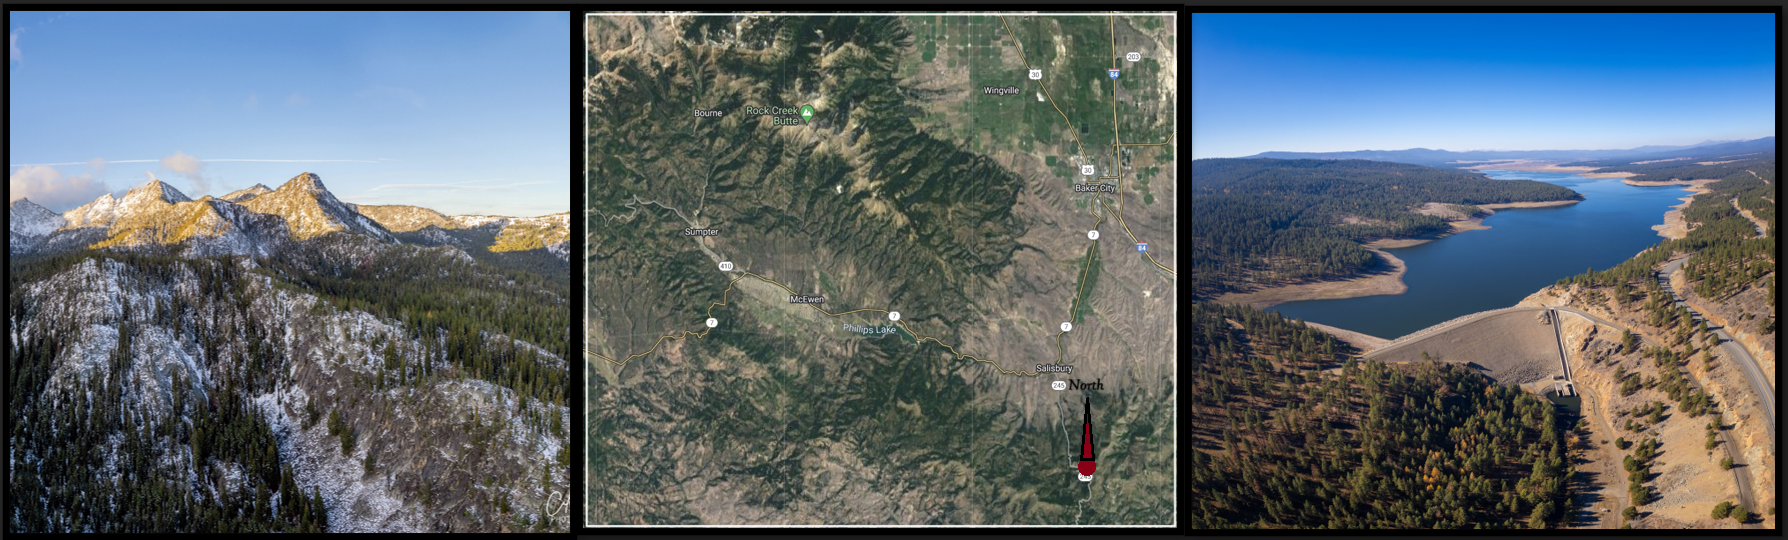
\includegraphics[width=\textwidth,height=5cm]{moun_mpa_res.png}
    \caption{Left image: portion of the Elkhorn Mountain range. Center image:  geographic area. Right image: Phillips Reservoir and Mason Dam. Drone images captured by Caleb Colton of Baker City, satellite image from \href{https://earth.google.com/web/@44.7920366,-117.99706468,1613.48832994a,83090.25038931d,35y,0h,0t,0r/data=OgMKATA}{Google Earth Engine} }
    \label{fig:enter-label}
\end{figure*}

\section{Data and Methods}

\textbf{The Data and Methods section should provide a \underline{quick} description of the datasets used in the project and the methodologies applied to analyze them. This section should included any preprocessing steps your team took to prepare the data for analysis. It should also outline the specific algorithms or models employed in the research, as well as any tools used. The goal is to give readers a clear understanding, ensuring that the project can be replicated.}

\def\arraystretch{1.5}
\begin{table}
\begin{center}
\small
\begin{tabular}{|c|c|c|}
\hline
\textbf{Features} & \textbf{Ranges and Units} & \textbf{Date Start} \\
\hline\hline
Water Volume &  \makecell{[-1159.91 to 81834.55] \\ acre-feet (af)} & 01/01/1968 \\
\hline
Water Discharge &  \makecell{[1.60 to 536.00] \\ cubic feet per second (cfs)} & 01/01/1968 \\
\hline
Temperature & \makecell{[-11.67 to 86.90] \\ Fahrenheit (degF)} & 11/7/1984\\
\hline
Precipitation & \makecell{[0.00 to  1.89] \\inches (in)} & 11/26/1980 \\
\hline
\end{tabular}
\caption{The data features pulled from the Hydromet data collection system. For this project, we utilize the change in water volume into our loss function. Notice how water volume can be negative and water discharge is never zero. \cite{Hydromet}}
\end{center}
\end{table}

\def\arraystretch{1.5}
\begin{table}[!h]
\begin{center}
\small
\begin{tabular}{|c|c|}
\hline
\textbf{Platform:} & Terra \\
\hline
\textbf{Sensor:} & MODIS \\
\hline
\textbf{Data Format:} & HDF-EOS2 \\
\hline
\textbf{Temporal Coverage:} & 24 February 2000 to present\\
\hline
\textbf{Temporal Resolution:} & 1 day \\
\hline
\textbf{Spatial Resolution:} &  5 km x 5 km \\
\hline
\textbf{Spatial Coverage:} & \makecell{N: 44.89, S: 44.55 \\ E: -117.76, W: -118.31}\\
\hline
\textbf{Image size:} & \makecell{7 x 12}\\
\hline
\hline
\textbf{Day CMG Snow Cover} & \makecell{The percentage of snowcovered land \\ 0-100: percent of snow in cell }\\
\hline
\textbf{Snow Spatial QA} & \makecell{Basic quality assurance indicator \\ 0: best, 1: good, 2:
ok, 3: poor, 4: other}\\
\hline
\end{tabular}
\caption{MODIS imagery data specifications and features pulled from the National Snow and Ice Data Center.}
\end{center}
\end{table}

\underline{\textbf{Example:}} Snow cover is detected using the Normalized Difference Snow Index (NDSI) in a preceding product (MOD10\_L2), which is ultimately carried forward to this product. Snowcovered land typically has a very high reflectance in visible bands (green \textbf{G} wavelengths, 545-565 nm) and very low reflectance in the shortwave infrared (\textbf{SWIR1} wavelengths 1628-1652 nm); the NDSI reveals the magnitude of this difference.~\cite{MODIS}

\begin{equation}
    \text{NDSI} = \frac{\text{G – SWIR1}}{\text{G + SWIR1}}
\end{equation}

Since the range for water level is in the tens of thousands, we normalized the water volume with the mean and standard deviation. Now water volume levels range between \textbf{[-1.42, 2.86]}.
%-------------------------------------------------------------------------

The incorporation of CNNs, positional encoding, and fully connected dense layers in a neural network architecture offers a comprehensive approach for addressing the research goals presented. CNNs excel in extracting spatial features and patterns from the MODIS imagery. The inclusion of positional encoding becomes crucial when dealing with time-series data, allowing the model to discern temporal dependencies and patterns. Simultaneously, fully connected dense layers are well-suited for recognizing global dependencies and correlations within non-spatial data, providing a holistic understanding of the overall context. 

To begin, we needed to take all of the datasets collected from these resources and develop a custom framework to input into our neural network design. We define a class called \texttt{Dataset\_30days\_2channels} for handling the time series data of water levels, positional encoding, and the MODIS imagery. The output of this class, for a single day, is a dictionary with the key structure: \texttt{dict\_keys([`image', `encoded\_time', `water\_level', `response'])}. The \texttt{`image'} is a tensor of shape (2 $\times$ 7 $\times$ 12) with the two channels corresponding to the snow and QA images for the current day, the \texttt{`encoded\_time'} is a vector of length 52 of the current day (whose length was randomly chosen), \texttt{`water\_level'} is the normalized water volume for the current day, and \texttt{`response'} is the normalized water level for $\Delta$t $= 30$ days in the future. 

The positional encoding is built into our dataset. It is beneficial after the CNN architecture and before entering the fully connected network because it introduces the notion of order of elements in the input sequence, providing the model with information about the relative positions of different features. This is particularly important for tasks where the order of elements matters, such as ours.

\begin{equation}
P(k, 2i) = \sin\left(\frac{k}{n^{\frac{2i}{d}}}\right)
\end{equation}
\begin{equation}
P(k, 2i+1) = \cos\left(\frac{k}{n^{\frac{2i}{d}}}\right)
\end{equation}

The variables are defined as:
\begin{itemize}
  \item \(\boldsymbol{k}\): Position of an object in the input sequence,\\ \(0 \leq \boldsymbol{k} \leq \boldsymbol{L}\)
  \item \(\boldsymbol{d}\): Dimension of the output embedding space (52 in our case)
  \item \(P(k, j)\): Position function for mapping a position in the input sequence to the index of the positional matrix
  \item \(\boldsymbol{n}\): User-defined scalar, set to 10,000 by industry standards ~\cite{Vaswani}
  \item \(\boldsymbol{i}\): Used for mapping to column indices \(0 \leq \boldsymbol{i} < 26\), where a single value of \(\boldsymbol{i}\) maps to both sine and cosine functions
\end{itemize}

Our final model architecture is called \texttt{`model\_30days\_2channels'}, which will be subsequently be referred to as \texttt{final\_model}. There are three convolutional layers to begin the structure.
Mean Squared Error (MSE) loss function is defined as the criterion for assessing the difference between predicted and actual values. Subsequently, an Adam optimizer is set up for \texttt{final\_model}. The optimizer is configured with a learning rate of \textbf{1e-3} and \textbf{L2} regularization, also known as weight decay, with a regularization strength of \textbf{5e-3}. The training process is then initiated using the \texttt{`Train\_model2'} function, which takes the model, optimizer, and other parameters such as the number of epochs (30 in this case), training and testing data loaders, and the device (e.g., CPU or GPU). The training function returns three traces: \texttt{loss\_trace} records the training loss over epochs, \texttt{test\_loss\_trace} records the testing loss, and \texttt{best\_index} indicates the index at which the model achieved the best performance on the test set.

%-------------------------------------------------------------------------
\section{Results}
\textbf{The Results section should present the key findings of your project in a clear manner. It should include any observations that directly address the chosen prompt. This section often features figures and descriptive text to highlight the most important outcomes. It's crucial to report the results objectively, without interpretation or discussion, leaving that for the subsequent section.}
The lowest loss we saw on the test set was around $0.133$ on epoch $8$. We see that the loss is increasing as epochs increase. An increase in MSE loss as epochs increase indicates that the model's predictions are deviating further from the actual values over time. 


\begin{figure}[h!]
  \centering
  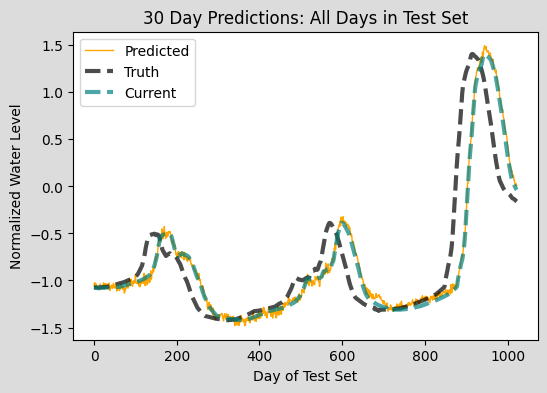
\includegraphics[width=.5\textwidth, height=6cm]{test_predictions.png}
  \caption{Predictions on the test set. Notice how the current water level at time $t$ and the prediction are closely linked, rather than the true water level at time $\Delta t$.}
  \label{fig:test_predictions}
\end{figure}

%-------------------------------------------------------------------------
\section{Conclusion}
\textbf{
The Conclusion section should summarize the main findings of your team's project, highlighting their significance and how they address the original research questions or objectives. Additionally, the conclusion may suggest areas for future research or acknowledge any limitations of the project that could be addressed in subsequent work. The goal is to provide a quick and concise closure to your research, reinforcing the importance of your findings.}
\vspace{0.5cm} 
\hrule
\vspace{0.5cm}

\textbf{Please see this link to our \href{...}{Submission Video}.} 

\textbf{Please see this link to our \href{...}{Google Colab Notebook}.} 

\vspace{0.5cm}
{\small
\bibliographystyle{alpha}
\bibliography{references}
}

\end{document}
